\documentclass{article}
\PassOptionsToPackage{numbers}{natbib}
\usepackage[main,final]{neurips_2026}

\usepackage[utf8]{inputenc} % allow utf-8 input
\usepackage[T1]{fontenc}    % use 8-bit T1 fonts
\usepackage{hyperref}       % hyperlinks
\usepackage{url}            % simple URL typesetting
\usepackage{booktabs}       % professional-quality tables
\usepackage{amsfonts}       % blackboard math symbols
\usepackage{nicefrac}       % compact symbols for 1/2, etc.
\usepackage{microtype}      % microtypography
\usepackage{xcolor}         % colors
\usepackage{amsmath}
\usepackage{graphicx} 
\usepackage{subcaption}

\title{GCT731 Homework \#1\\Piano Music Transcription}

\author{%
  Joo Eun Lim (20244418) \\
  Graduate School of Culture Technology, KAIST
}

\begin{document}

\maketitle

\section{Introduction}
Automatic music transcription involves converting acoustic signals into symbolic formats such as MIDI. Transcribing piano music is particularly challenging due to its complex overlapping notes and polyphony. This project implements the onsets and frames model which predicts note initiation and sustained duration separately to avoid errors like note fragmentation. The convolutional design originates from bay et al. \cite{bay2009evaluation}, while the dual objective strategy for onsets and frames is based on the framework established by Hawthorne et al. \cite{hawthorne2018onsetsframesdualobjectivepiano}.

This report follows four stages, beginning with an architectural review and hyperparameter tuning. It then transitions to implementing bidirectional LSTMs and establishing hierarchical links between predictions to improve temporal accuracy. Finally, potential innovations like pitch aligned representations or data augmentation are explored. All experiments use a 170 piece subset of the MAESTRO dataset, split into 100 training, 20 validation, and 50 test pieces to understand how structured dependencies lead to professional level transcription.

Performance is evaluated primarily using Note-level F1-score, precision, and recall. These metrics treat notes as discrete events defined by pitch and onset, providing a musically meaningful assessment \cite{bay2009evaluation}. Following standard conventions, a predicted note is correct only if the pitch matches the ground truth and the onset falls within a $\pm$50ms tolerance \cite{hawthorne2018onsetsframesdualobjectivepiano}. While frame-level F1, precision, and recall are also available, such metrics often overestimate performance through spectral overlap and fail to capture note boundaries. Consequently, Note-level metrics are utilized exclusively to provide a rigorous benchmark for symbolic transcription accuracy.

\section{Question 1: Review the Baseline Model}
The baseline model corresponds to the non-recurrent dual-stack CNN configuration described in the ablation studies of Hawthorne et al. \cite{hawthorne2018onsetsframesdualobjectivepiano}. This version removes the temporal smoothing provided by LSTMs to evaluate the fundamental performance of the feature extraction layers. In this setup, the frame stack predicts the sustained state of notes while the onset stack identifies the attack transience at the beginning of each musical event. Figure \ref{fig:baseline_arch} illustrates the complete structure of this architecture including the connectivity between layers and the corresponding tensor sizes at each stage. This visual representation serves as the primary map for understanding how input audio is transformed into piano-roll probabilities.

\subsection{Parameters and Variables}The hyper-parameters and dimensions defining the overall model shown in the architecture diagram are summarized in Table \ref{tab:dimensions}.

\begin{table}[ht]
\centering
\caption{Specific hyper-parameters and tensor dimensions used in the baseline model.}
\label{tab:dimensions}
\begin{tabular}{llll}
\toprule
Parameter & Value & Variable Name & Description \\ \midrule
$B$ & 16 & \texttt{batch\_size} & Batch size for parallel processing \\
$L$ & 102,400 & \texttt{sequence\_length} & Samples in the raw input waveform \\
$T$ & 200 & - & Number of temporal frames \\
$F$ & 229 & \texttt{N\_MELS} & Log-Mel filterbank bins \\
$C$ & 24 & \texttt{cnn\_unit} & Base channel depth \\
$C'$ & 64 & \texttt{fc\_unit} & Hidden projection dimension \\
$C''$ & 88 & - & Output keys (MIDI range) \\ \bottomrule
\end{tabular}
\end{table}




\subsection{Processing Pipeline}

\begin{figure}
\centering
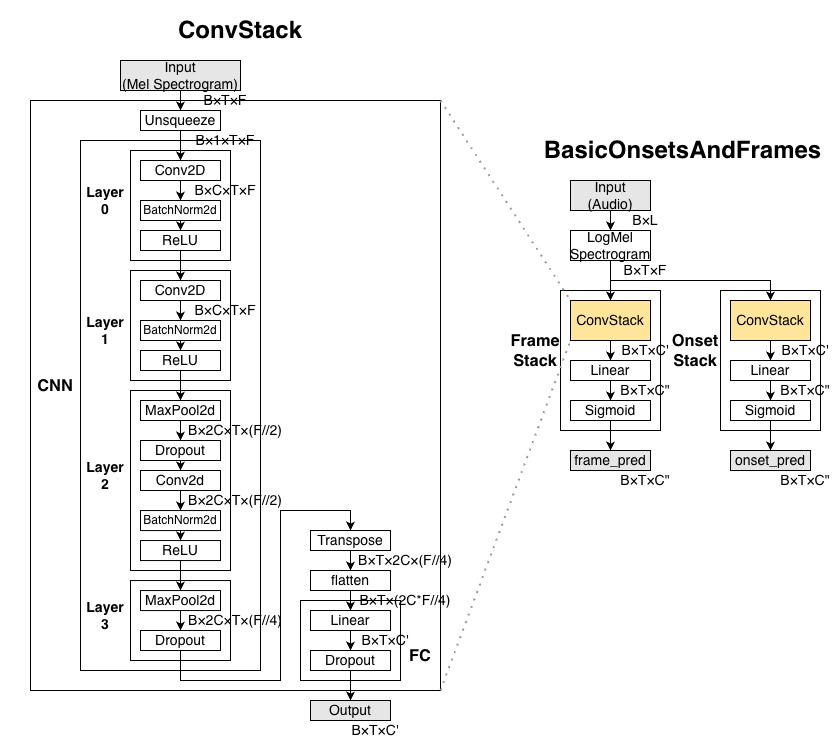
\includegraphics[width=1\linewidth]{imgs/hw1_BasicOnsetsAndFrames.jpg}
\caption{Architecture overview of the baseline model as adapted from \cite{hawthorne2018onsetsframesdualobjectivepiano}.}
\label{fig:baseline_arch}
\end{figure}

\subsubsection[Pre-processing]{Pre-processing ($\mathbb{R}^{B \times L} \rightarrow \mathbb{R}^{B \times 1 \times T \times F}$)}
The raw waveform is converted into a time-frequency representation suitable for 2D spatial feature extraction.
\begin{itemize}
    \item \textbf{Input ($\mathbb{R}^{B \times L}$)}: The model receives a batch of raw audio segments with batch size $B$ and sample length $L$.
    \item \textbf{Log-Mel Spectrogram ($\mathbb{R}^{B \times L} \rightarrow \mathbb{R}^{B \times T \times F}$)}: The 1D signal is mapped to a 2D plane via STFT and Mel-filterbanks, resulting in $T$ time steps and $F$ mel bins. Log-scaling is applied to normalize the dynamic range.
    \item \textbf{Unsqueeze ($\mathbb{R}^{B \times T \times F} \rightarrow \mathbb{R}^{B \times 1 \times T \times F}$)}: Adds a singleton dimension to the tensor, allowing the mel-spectrogram to be treated as a single-channel image for subsequent 2D convolutions.
\end{itemize}

\subsubsection[Frame and Onset Stack]{Frame and Onset Stack ($\mathbb{R}^{B \times 1 \times T \times F} \rightarrow \mathbb{R}^{B \times T \times C'}$)}
This stage extracts hierarchical spectral-spatial features while preserving the temporal axis for frame-level prediction.
\begin{itemize}
    \item \textbf{CNN Layers ($\mathbb{R}^{B \times 1 \times T \times F} \rightarrow \mathbb{R}^{B \times 2C \times T \times F/4}$)}: Hierarchical features are extracted via a four-layer convolutional stack. Layers 0 and 1 expand the channel depth to $C$ using $3 \times 3$ Conv2D (padding=1), which preserves the spatial resolution according to the identity $X // 1 - (3-1) + 2 = X$. Layer 2 then reduces the frequency resolution to $F/2$ through a MaxPool2d(1, 2) operation while further expanding the depth to $2C$ with an additional Conv2D layer. Finally, Layer 3 performs a second frequency compression to $F/4$ using MaxPool2d(1, 2). Integrated throughout these layers are BatchNorm2D for channel-wise normalization, ReLU for non-linearity, and Dropout for robust regularization. Crucially, the time dimension $T$ is kept constant across all layers to facilitate precise one-to-one frame matching for transcription.
    
    \item \textbf{Feature Reorganization ($\mathbb{R}^{B \times 2C \times T \times F/4} \rightarrow \mathbb{R}^{B \times T \times (2C * F/4)}$)}: The tensor is transposed to swap Channel and Time dimensions to align features chronologically. It is then flattened to size $ 2C * F/4$ to consolidate multi-channel spectral attributes into a single dense vector, enabling sequential modeling of the collapsed spectral data.
    
    \item \textbf{FC Part ($\mathbb{R}^{B \times T \times (2C * F/4)} \rightarrow \mathbb{R}^{B \times T \times C'}$)}: The flattened features are projected through a Linear layer into a latent space of size $C'$, followed by a final Dropout layer to refine the representation before sequence modeling.
\end{itemize}

\subsubsection[Prediction Head]{Prediction Head ($\mathbb{R}^{B \times T \times C'} \rightarrow \mathbb{R}^{B \times T \times C''}$)}
The high-dimensional features are mapped into the final label space for pitch-wise transcription.
\begin{itemize}
    \item \textbf{Latent Projection ($\mathbb{R}^{B \times T \times C'} \rightarrow \mathbb{R}^{B \times T \times C''}$)}: A Linear layer maps the latent features from $C'$ to the final prediction space $C''$ (e.g., 88 keys), projecting the abstract features into pitch-specific logit values.
    \item \textbf{Sigmoid Activation ($\mathbb{R}^{B \times T \times C''} \rightarrow \mathbb{R}^{B \times T \times C''}$)}: An element-wise sigmoid function is applied to produce independent probabilities $\hat{\mathbf{y}}_t \in [0, 1]^{C''}$ for $C''=88$ keys at each time step $t$.
    \item \textbf{Output} ($\mathbb{R}^{B \times T \times C''}$): This process yields \texttt{frame\_pred} and \texttt{onset\_pred}, indicating respectively whether a key is sustained or if a new note has started.
\end{itemize}


\section{Question 2: Run the Baseline Model}
The performance of the baseline model is evaluated by systematically investigating five key hyperparameters: sequence length ($L$), CNN units ($C$), fully connected units ($fc\_unit$), learning rate ($\eta$), and weight decay ($\lambda$). The primary objective is to identify the configuration that yields the highest validation accuracy, with the findings subsequently verified through F1-score, precision, and recall to ensure robust transcription performance.

\subsection{Hypotheses}
The anticipated effects of data framing, model capacity, and optimization strategies are outlined below.
\begin{itemize}
    \item \textbf{Temporal Resolution}: A shorter sequence length $L$ is expected to capture rapid temporal transients more effectively by preventing information loss associated with temporal averaging in longer frames.
    \item \textbf{Model Capacity}: Increasing the number of CNN units $C$ and fully connected units $fc\_unit$ is anticipated to provide the representational complexity necessary to adapt to the underlying audio distribution.
    \item \textbf{Optimization Stability}: It is hypothesized that a smaller learning rate $\eta$ and the inclusion of weight decay $\lambda$ will offer superior stability and generalization, resulting in the highest validation accuracy.
\end{itemize}

\subsection{Experimental Settings}
The experimental design consists of two structured sweeps to evaluate architectural and optimization choices.

\subsubsection{Experiment 1: Dataset and Model Hyperparameters}
A grid search is performed to identify the optimal architecture and data framing. The tested parameter sets are defined as follows:
\begin{itemize}
    \item \textbf{Sequence Lengths ($L$)}: $\{51200, 102400, 204800\}$
    \item \textbf{CNN Units ($C$)}: $\{12, 24, 48\}$
    \item \textbf{FC Units ($fc\_unit$)}: $\{32, 64, 128\}$
\end{itemize}
Fixed parameters include a batch size of 16, $\eta = 10^{-3}$, $\lambda = 0$, and 10 epochs of 1000 optimizer steps each (10{,}000 total iterations).

\subsubsection{Experiment 2: Training Hyperparameters}
Using the optimal architecture from the previous experiment, optimization settings are investigated to refine convergence. The tested parameter sets are defined as follows:
\begin{itemize}
    \item \textbf{Learning Rates ($\eta$)}: $\{10^{-4}, 10^{-3}, 10^{-2}\}$
    \item \textbf{Weight Decays ($\lambda$)}: $\{0.0, 10^{-4}, 10^{-3}\}$
\end{itemize}
Fixed parameters are set to the optimal values from Experiment 1 ($L=51200, C=48, fc\_unit=128$) with a batch size of 16 and 10 epochs of 1000 optimizer steps each.



\subsection{Results}

The following outcomes detail the performance metrics, where the F1-score, precision, and recall were evaluated at the epoch corresponding to the minimum validation loss. 

\begin{figure}[ht]
    \centering
    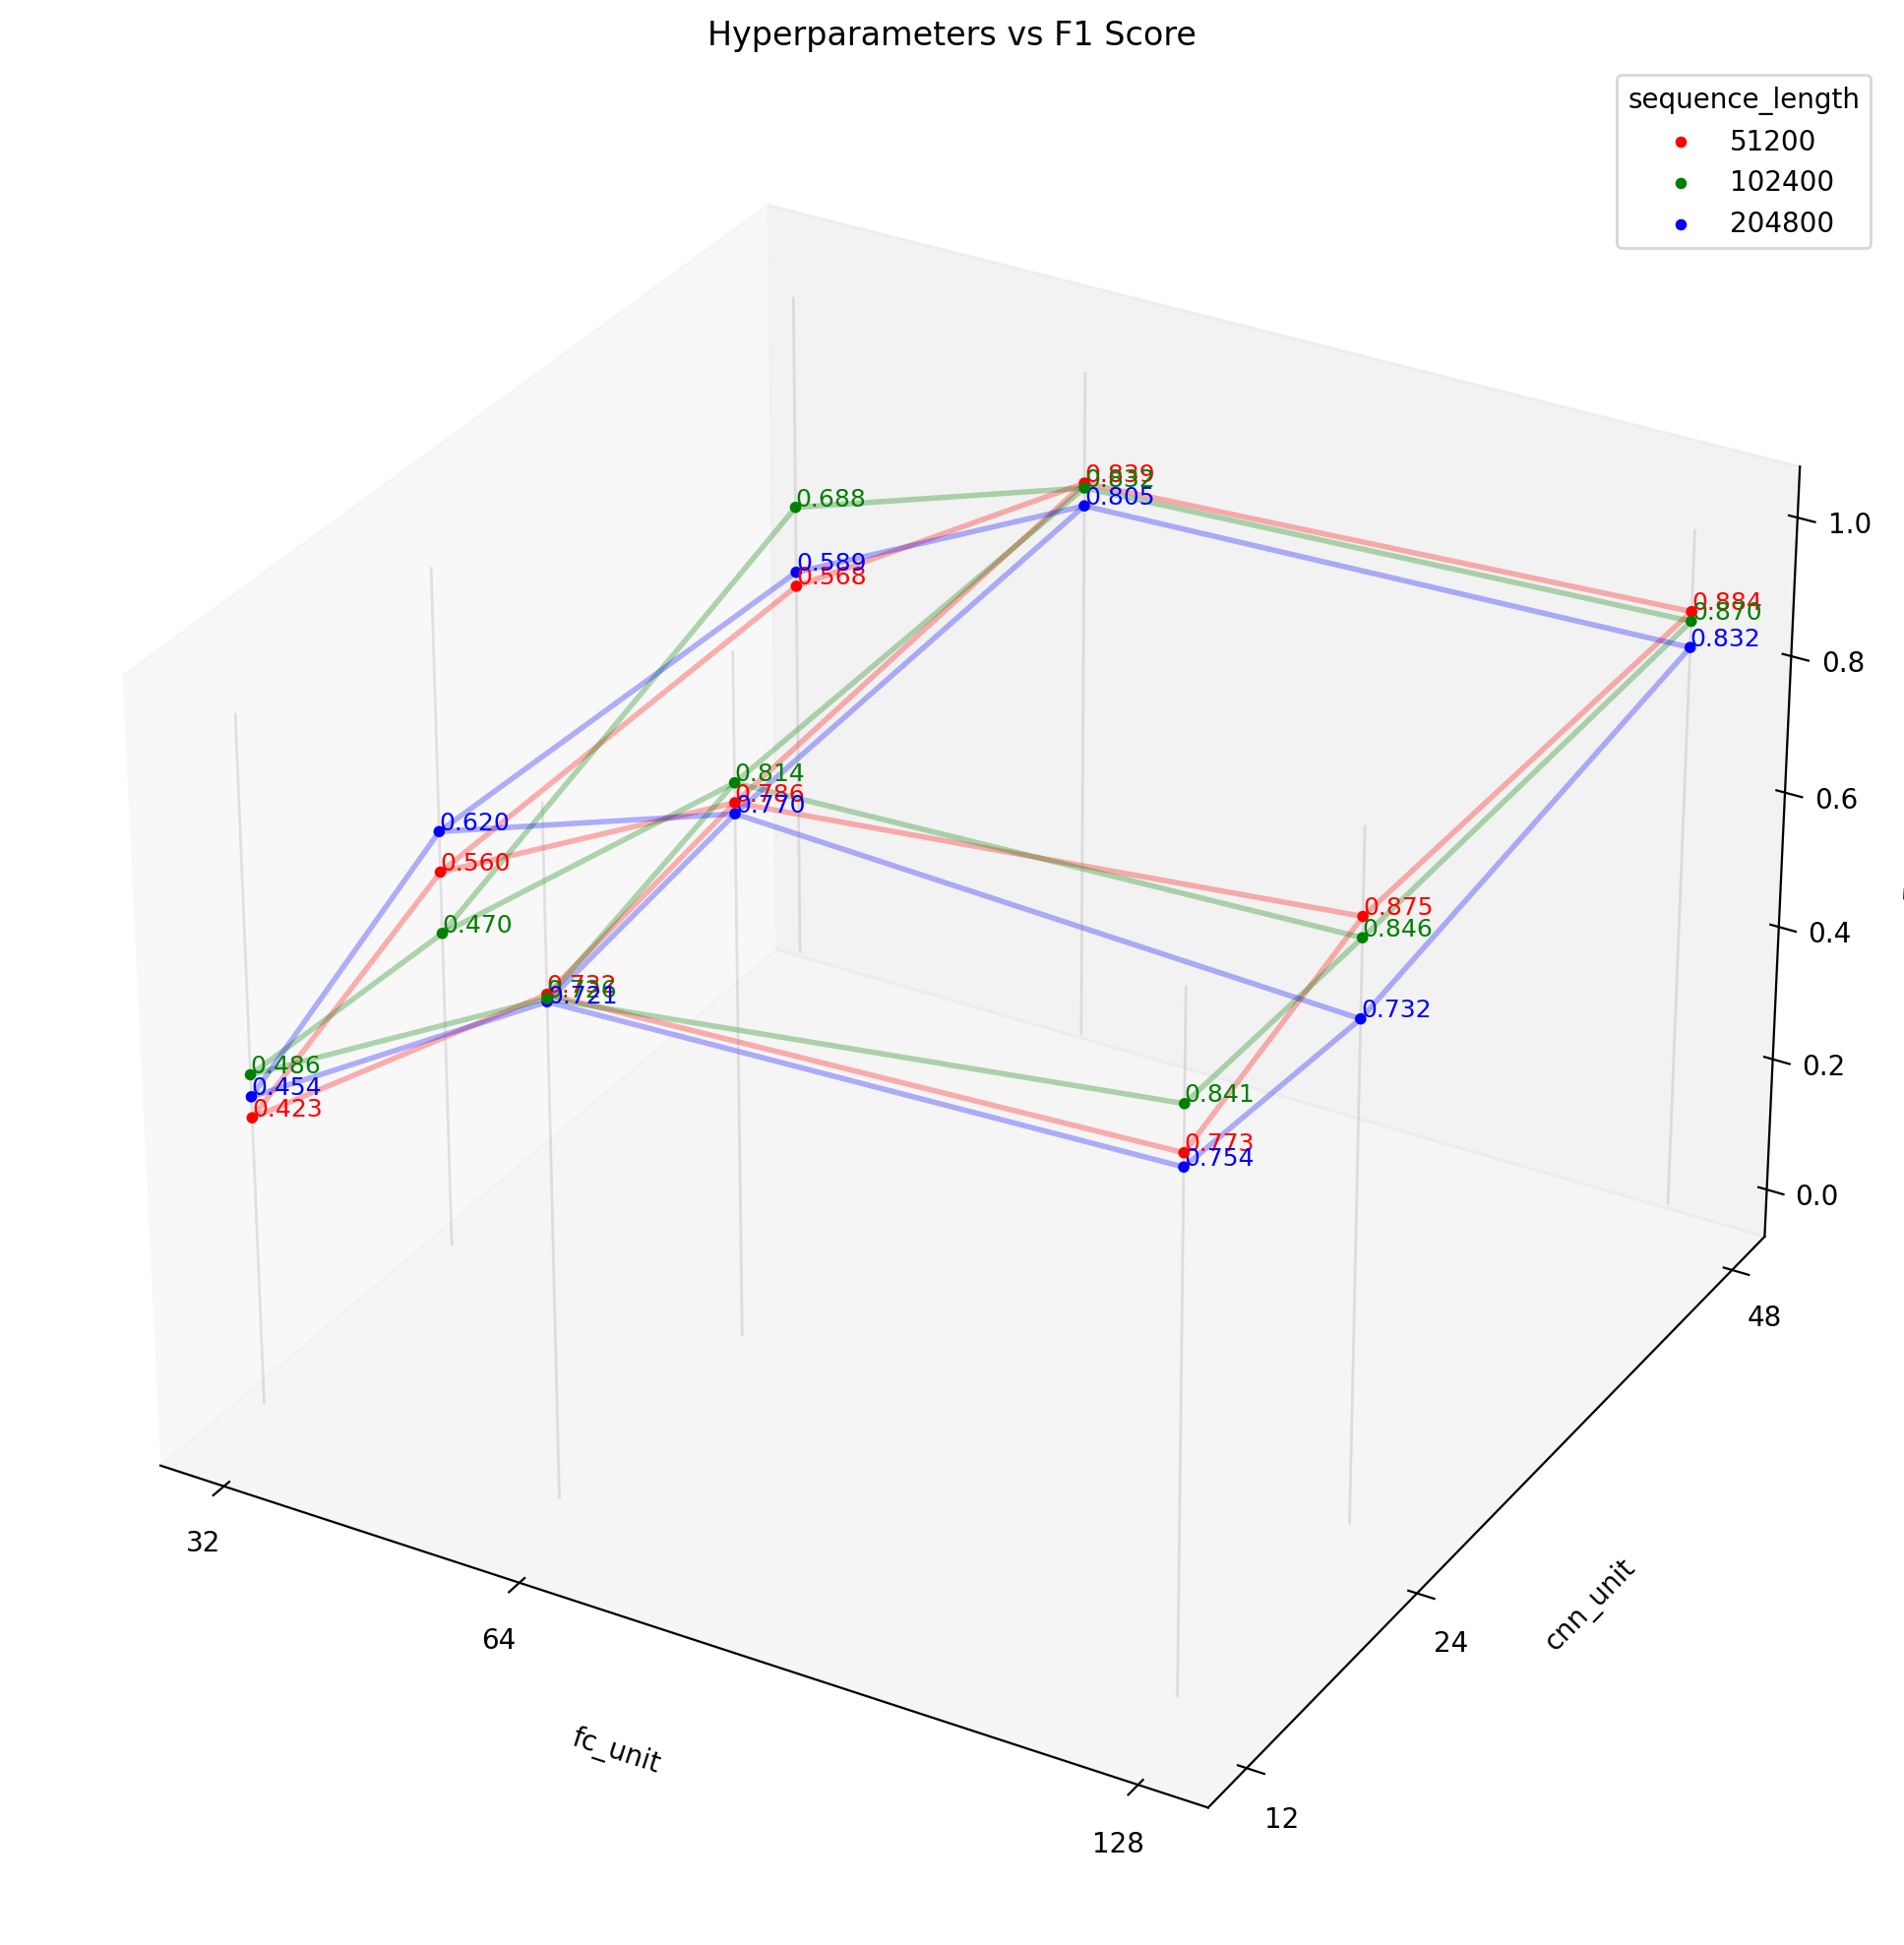
\includegraphics[width=0.8\linewidth]{imgs/hw1_exp1_f1.png}
    \caption{Performance evaluation of F1-scores across varying sequence lengths and model capacities.}
    \label{fig:exp1_results}
\end{figure}


\subsubsection{Experiment 1: Dataset and Model Hyperparameters}

The evaluation in Figure \ref{fig:exp1_results} shows that peak performance across all metrics is achieved with the shortest sequence length of $L=51200$ and the maximum model capacity where $C=48$ and $fc\_unit=128$. A consistent trend of improved scores is observed as the number of CNN and fully connected units increases. While the smallest sequence length generally yields the best results, the ranking of $L$ values fluctuates when model capacity is low. In these smaller configurations, larger sequence lengths occasionally outperform smaller ones, though this inconsistency is resolved as the model capacity grows. 

Additionally, as illustrated in Figure \ref{fig:performance_detailed}, the comparative analysis of precision and recall indicates that recall has a more substantial impact on the overall performance trends. While precision exhibits relatively stable behavior across different configurations, recall shows more significant variance, suggesting that the tested parameters primarily influence the ability of the model to capture note events rather than the accuracy of the identified segments.

\begin{figure}[ht]
    \centering
    \begin{subfigure}[b]{0.48\textwidth}
        \centering
        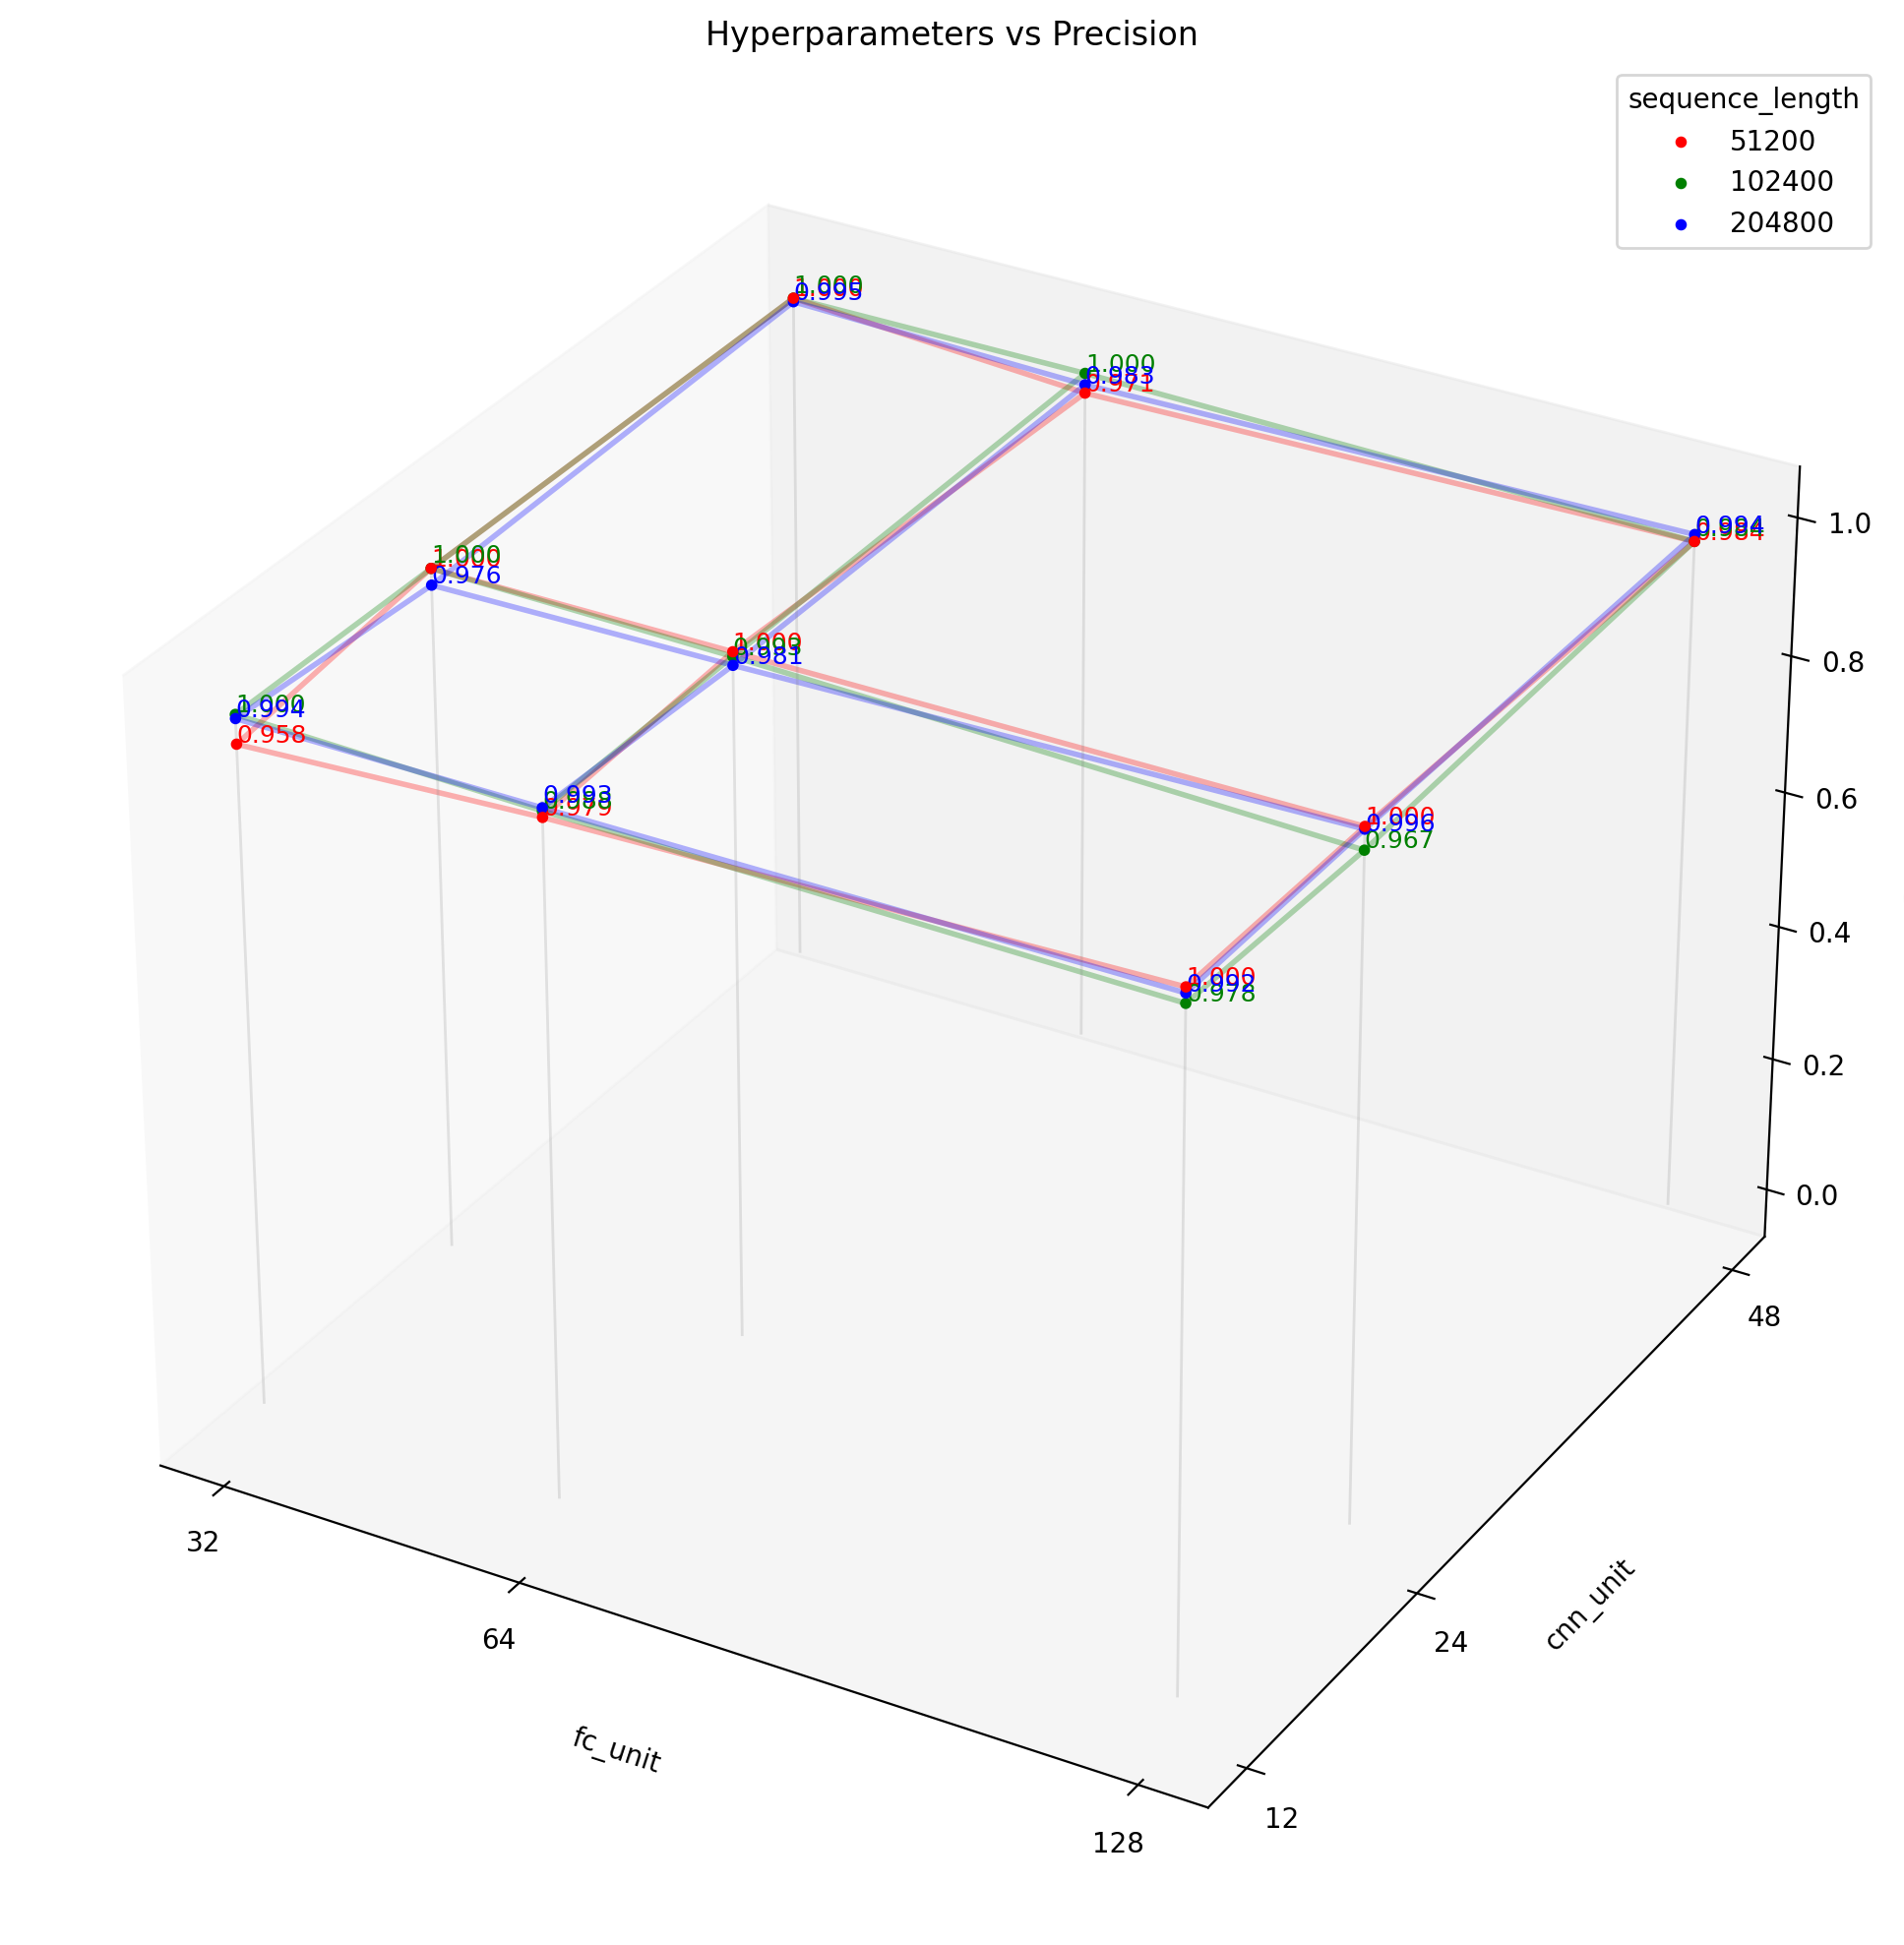
\includegraphics[width=\linewidth]{imgs/hw1_exp1_pre.png}
        \caption{Precision performance.}
        \label{fig:precision}
    \end{subfigure}
    \hfill
    \begin{subfigure}[b]{0.48\textwidth}
        \centering
        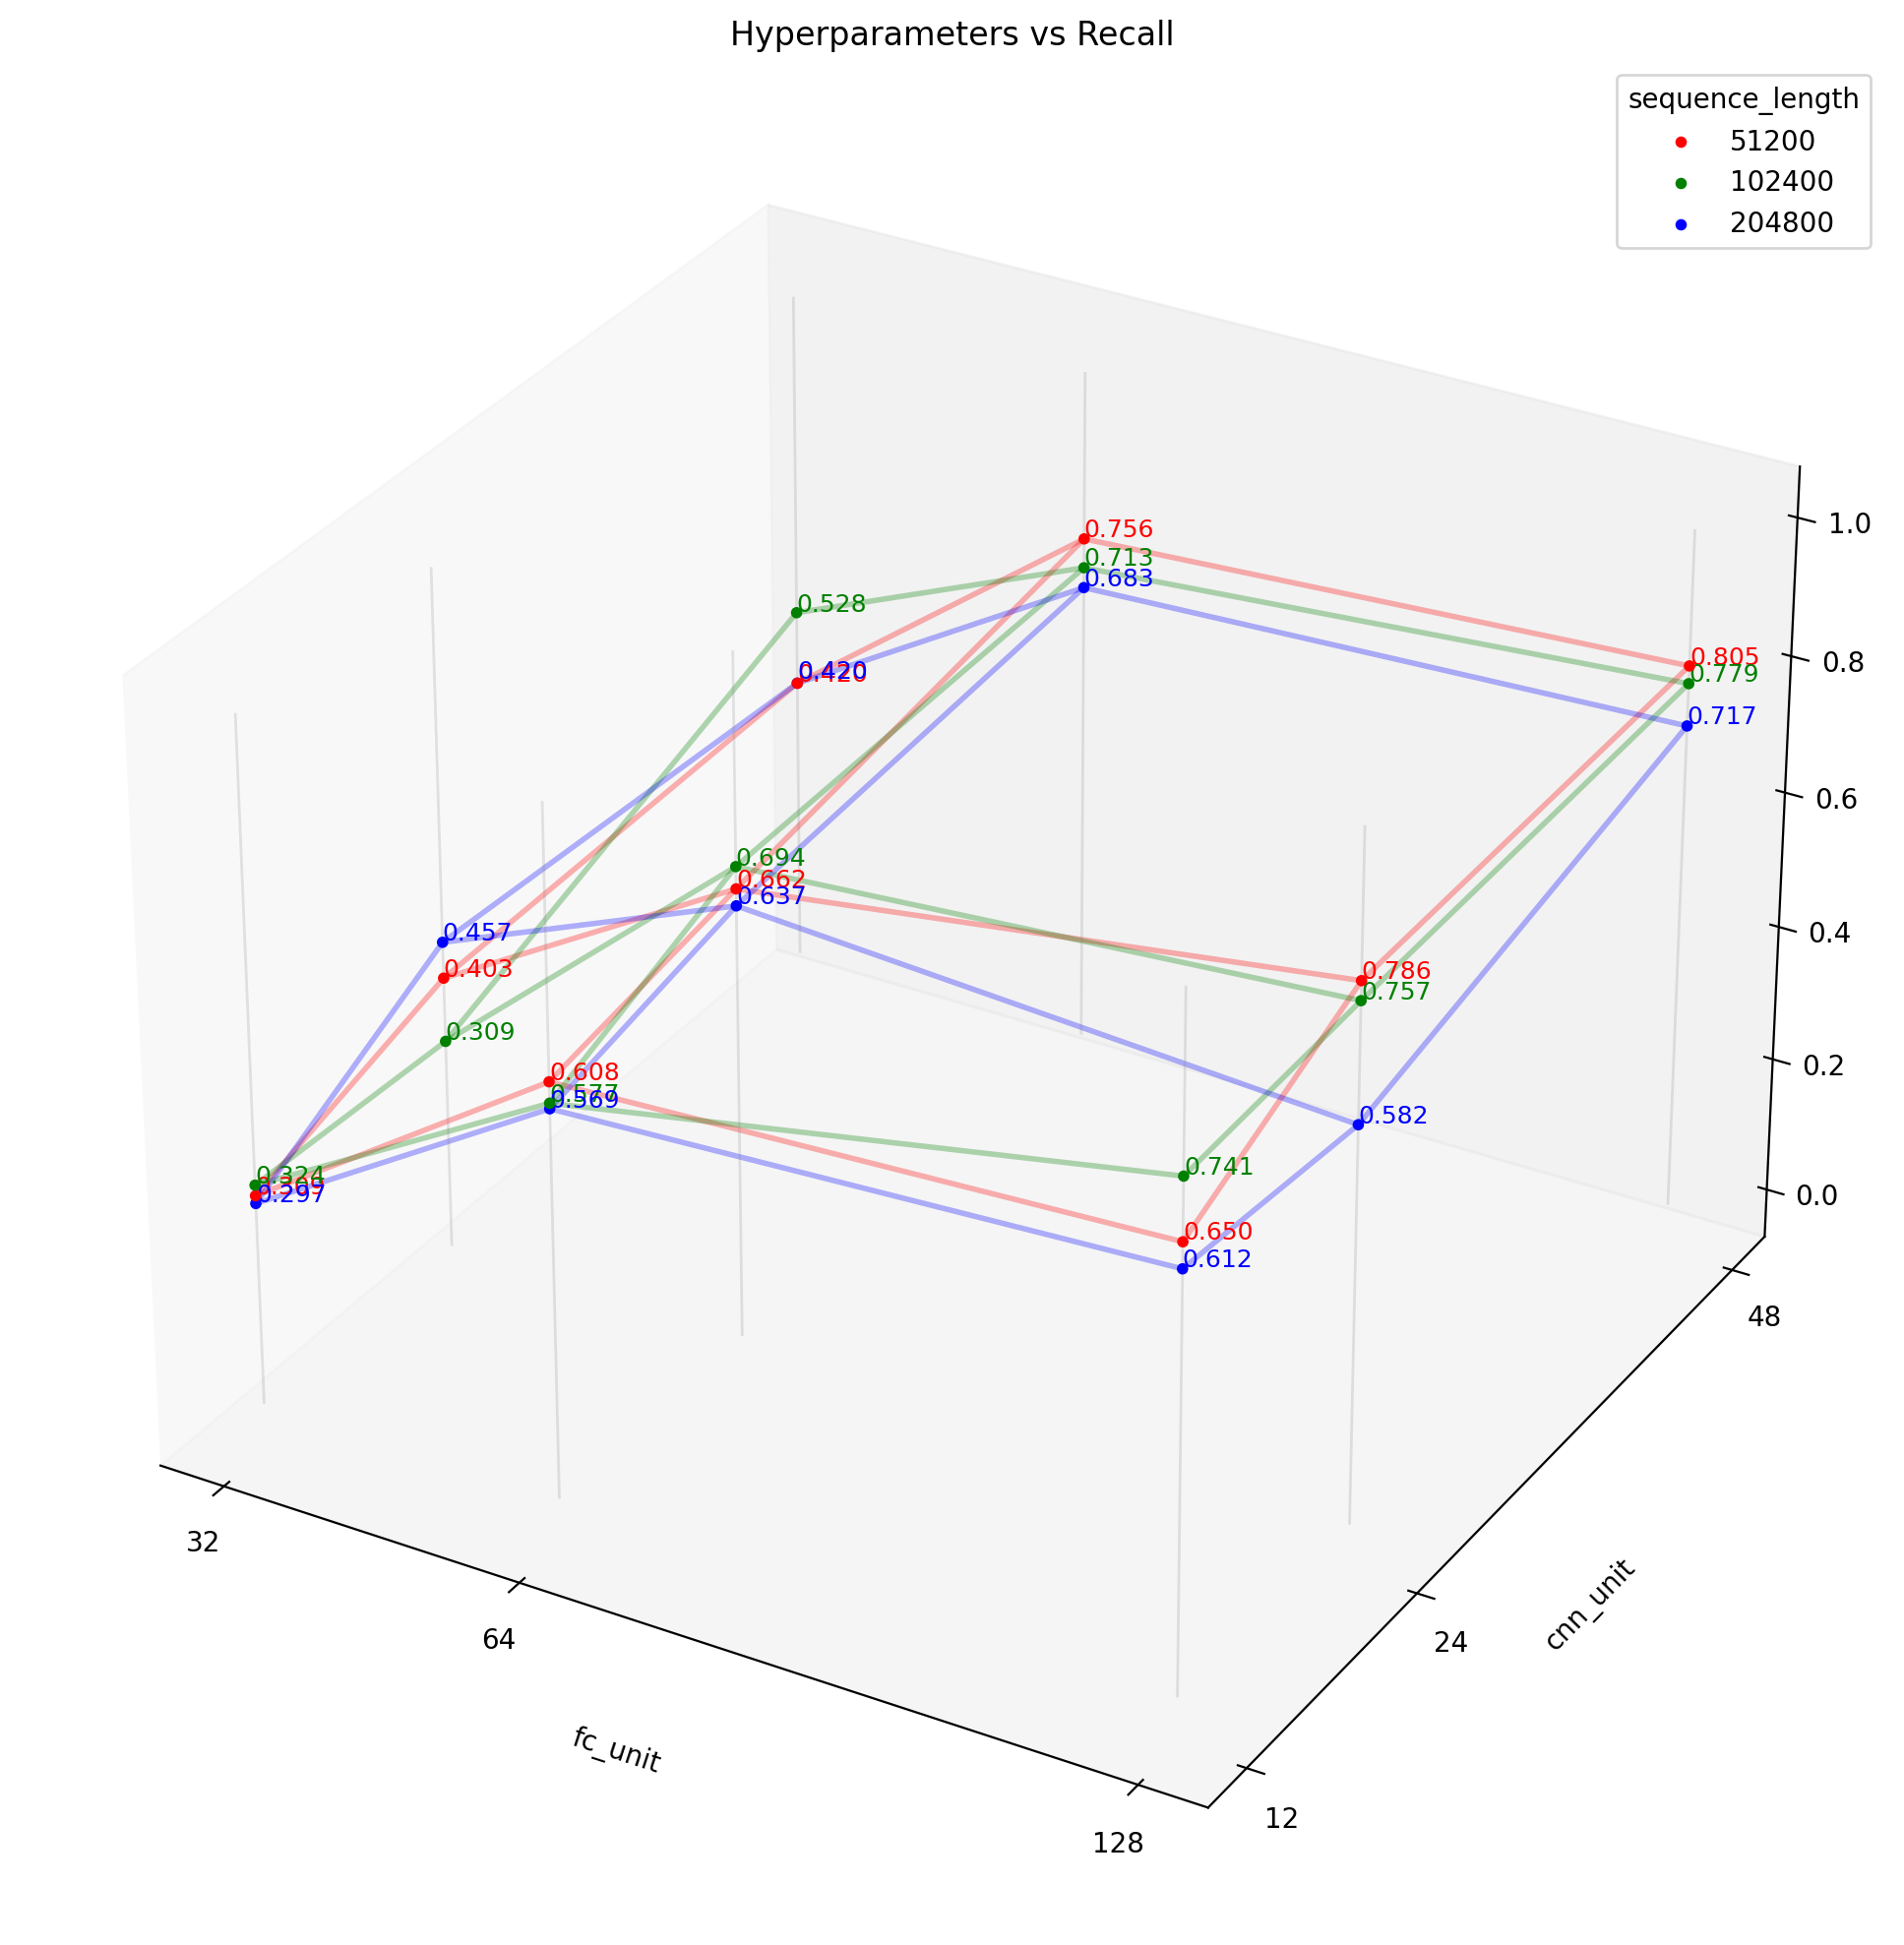
\includegraphics[width=\linewidth]{imgs/hw1_exp1_rec.png}
        \caption{Recall performance.}
        \label{fig:recall}
    \end{subfigure}
    \caption{Detailed performance analysis of the model in terms of (a) Precision and (b) Recall across dataset splits.}
    \label{fig:performance_detailed}
\end{figure}


\subsubsection{Experiment 2: Training Hyperparameters}

The evaluation results illustrated in Figure \ref{fig:exp2_results} indicate that the highest F1-score, precision, and recall are achieved at a learning rate of $\eta = 10^{-3}$ and a weight decay of $\lambda = 0$ around epoch 10. Across all these performance metrics, lower weight decay values and the absence of regularization lead to more favorable scoring trends throughout the training process. Although lower learning rates generally exhibit more stable and positive trends for all three metrics, the configuration using $\eta = 10^{-3}$ in combination with zero weight decay provides the most effective overall performance within the observed training duration.

While the overall trends for F1-score, precision, and recall are similar, a distinct temporal pattern is observed where precision reaches high values relatively easily. This is followed by a subsequent development in recall, suggesting that the model initially learns to identify clear note events with high certainty before gradually improving its capacity to detect a wider range of note instances.

\begin{figure}[ht]
    \centering
    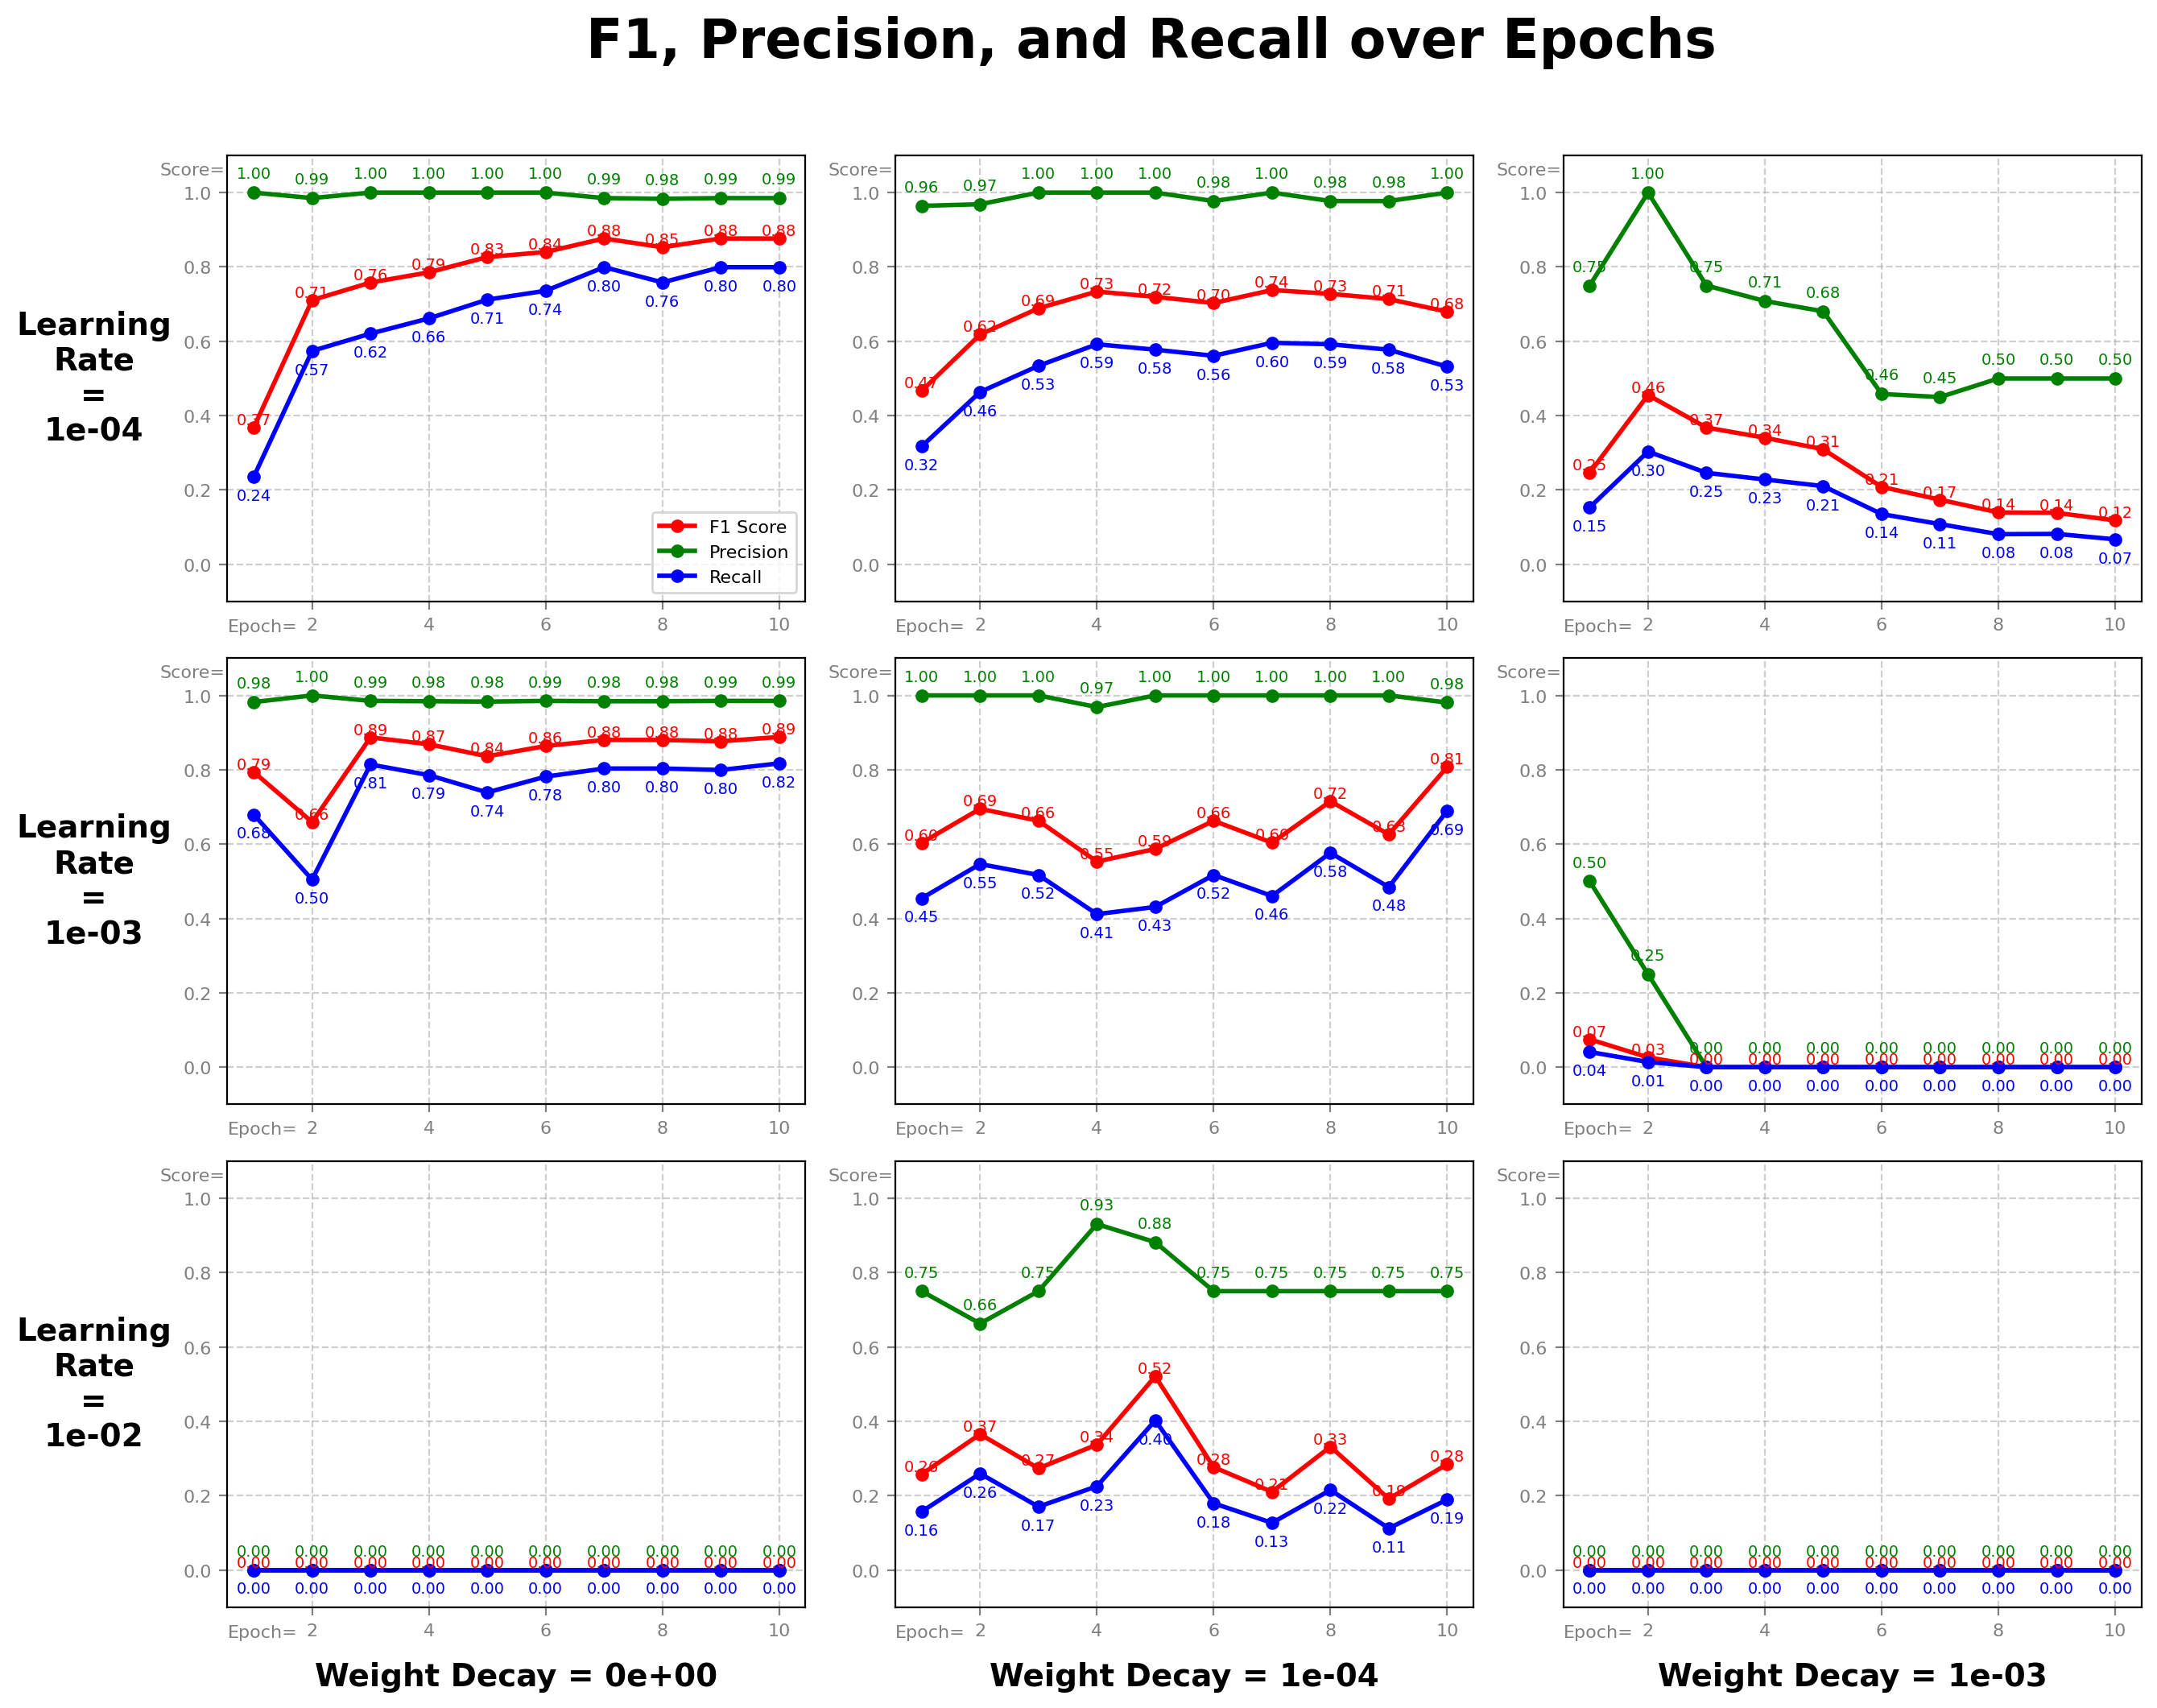
\includegraphics[width=1\linewidth]{imgs/hw1_exp2.png}
    \caption{Trends of F1-score, precision, and recall across different learning rates and weight decay settings.}
    \label{fig:exp2_results}
\end{figure}

\subsection{Discussion}
The experimental results provide a comprehensive evaluation of the initial hypotheses while revealing nuanced interactions between model capacity and temporal resolution.

\begin{itemize}
    \item \textbf{Temporal Resolution and Model Capacity (Hypotheses Confirmed)}: The results validate that shorter sequence lengths such as $L=51200$ are superior for capturing rapid transients. However, the observed fluctuation in the ranking of $L$ when model capacity is low suggests a dependency between resolution and representational power. Fine temporal features appear to require a minimum threshold of CNN and fully connected units to be effectively processed, as the benefits of shorter sequences only become consistent as model capacity increases.
    
    \item \textbf{Optimization Strategy (Hypothesis Contradicted)}: The findings contradict the hypothesis that smaller learning rates and higher weight decay would improve generalization. Instead, a moderate learning rate of $\eta = 10^{-3}$ and the absence of weight decay ($\lambda = 0$) proved most effective. This indicates that for this baseline configuration, explicit regularization may overly constrain the learning process, and sufficient gradient steps are necessary to reach optimal performance within a limited number of epochs.
    
    \item \textbf{Learning Dynamics and Metric Sensitivity}: A significant observation is that recall serves as the primary driver for overall performance gains, showing much higher variance across configurations than precision. The temporal pattern during training, where precision reaches high values early followed by a gradual increase in recall, suggests that the model first prioritizes the certain identification of clear note events. The subsequent improvement in F1-score is largely determined by the model's expanding capacity to detect a wider range of note instances without significantly sacrificing accuracy.
\end{itemize}

\section{Question 3: Implement the Onsets and Frames Model}
In comparison to the baseline implementation in the previous section, the full Onsets and Frames model is developed to incorporate hierarchical dependencies and temporal context. The efficacy of this expanded architecture is explored through the tuning of new hyperparameters, specifically the RNN hidden unit size ($R$), and a structural ablation study, isolating the individual and synergistic effects of each component on transcription performance. The findings are verified using F1-score, precision, and recall.


\begin{table}[ht]
\centering
\caption{Specific hyper-parameters and tensor dimensions used in the full model.}
\label{tab:dimensions_full}
\begin{tabular}{llll}
\toprule
Parameter & Value & Variable Name & Description \\ \midrule
$B$ & 16 & \texttt{batch\_size} & Batch size for parallel processing \\
$L$ & 51{,}200 & \texttt{sequence\_length} & Samples in the raw input waveform \\
$T$ & 100 & - & Number of temporal frames \\
$F$ & 229 & \texttt{N\_MELS} & Log-Mel filterbank bins \\
$C$ & 48 & \texttt{cnn\_unit} & Base channel depth \\
$C'$ & 128 & \texttt{fc\_unit} & Hidden projection dimension \\
$C''$ & 88 & - & Output keys (MIDI range) \\
$R$ & 128 & \texttt{rnn\_unit} & RNN hidden unit size \\ \bottomrule
\end{tabular}
\end{table}

\subsection{Architecture}


\begin{figure}[ht]
    \centering
    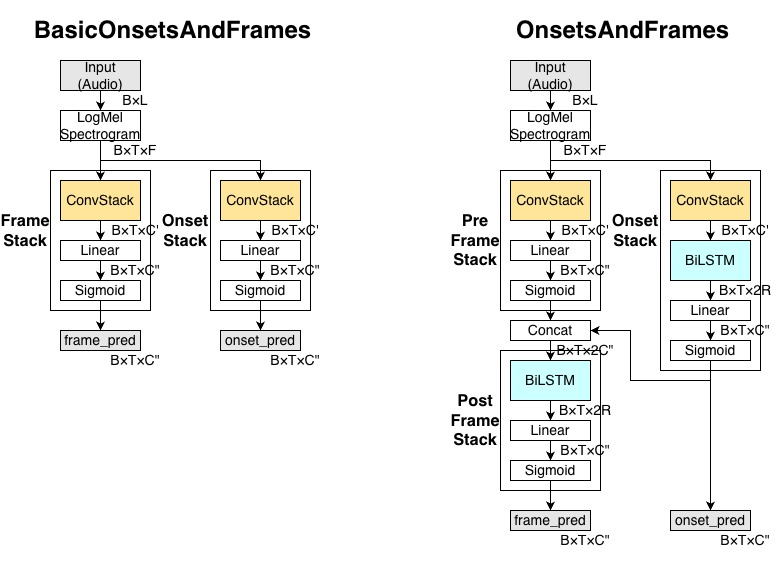
\includegraphics[width=1\linewidth]{imgs/hw1_OnsetsAndFrames.jpg}
    \caption{Architectural comparison between the baseline BasicOnsetsAndFrames and the full OnsetsAndFrames model, highlighting the introduction of Bi-LSTMs and hierarchical concatenation.}
    \label{fig:arch_comparison}
\end{figure}

\begin{figure}[ht]
    \centering
    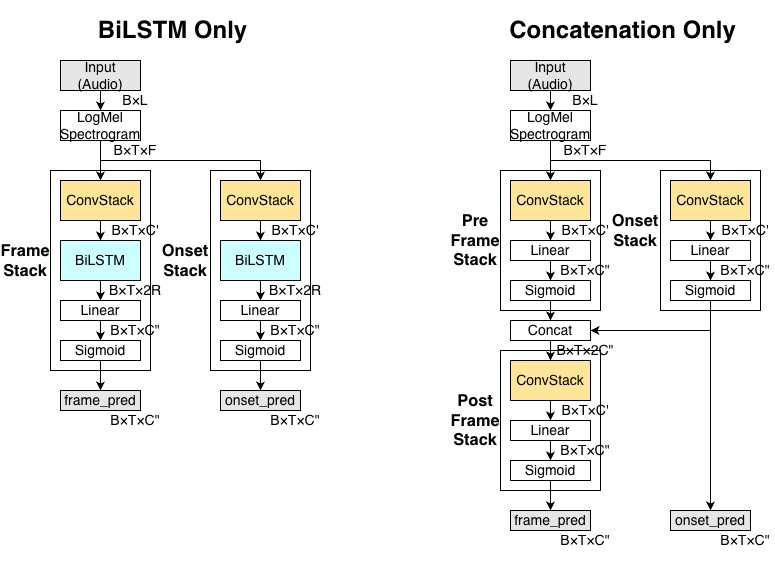
\includegraphics[width=1\linewidth]{imgs/hw1_Ablations.jpg}
    \caption{Structural variations for ablation study: BiLSTMOnly, and ConcatOnly models.}
    \label{fig:ablations}
\end{figure}
The Onsets and Frames model evolves from the baseline by integrating recurrent temporal context and hierarchical conditioning, as illustrated in Figure~\ref{fig:arch_comparison}. While both the baseline and the advanced model utilize a dual-stack system for onset and frame prediction, the full model introduces Bi-directional LSTMs (Bi-LSTMs) and hierarchical concatenation. Specifically, onset predictions are concatenated into the frame stack's input, ensuring that sustainment predictions are logically informed by detected onset events.

To isolate the impact of each architectural feature, four structural variations are evaluated: \textit{Basic}, \textit{BiLSTMOnly}, \textit{ConcatOnly}, and the full \textit{OnsetsAndFrames} model. The structural variations of these ablation variants are depicted in Figure~\ref{fig:ablations}, and the corresponding hyper-parameters and tensor dimensions are summarized in Table~\ref{tab:dimensions_full}.


\subsection{Hypotheses}
The anticipated effects of temporal capacity and structural hierarchy are outlined below.
\begin{itemize}
    \item \textbf{RNN Capacity}: Increasing the number of RNN hidden units ($R$) is expected to enhance the model's ability to learn complex temporal dependencies, leading to higher transcription accuracy.
    \item \textbf{Structural Ablation}: It is hypothesized that the addition of Bi-LSTMs for temporal modeling and hierarchical concatenation for onset-priors will independently improve performance relative to the baseline. Furthermore, the integration of both features in the full model is expected to yield the highest performance through a synergistic effect, combining long-term sequential context with logical constraints on note sustainment.
\end{itemize}

\subsection{Experimental Settings}
The experimental design evaluates the impact of temporal modeling and architectural variations through two structured approaches. The tested parameters and model configurations are defined as follows:

\begin{itemize}
    \item \textbf{RNN Hidden Sizes ($R$)}: $\{32, 64, 128\}$
    \item \textbf{Model Variants}: \textit{Basic}, \textit{BiLSTMOnly}, \textit{ConcatOnly}, and the full \textit{OnsetsAndFrames}
\end{itemize}

For both experiments, the training configuration was maintained with a batch size ($B$) of 16 and a sequence length ($L$) of 51,200. The model architecture utilized 48 CNN units ($C$) and 128 fully connected units ($fc\_unit$). Optimization was conducted using a learning rate ($\eta$) of $10^{-3}$ and a weight decay ($\lambda$) of $0.0$, with each model trained for a total of 20 epochs. In the structural ablation study, the RNN hidden size was fixed at $R = 128$ for the variants where applicable.

\subsection{Results}

The following outcomes detail the performance metrics, where the F1-score, precision, and recall were evaluated at the epoch corresponding to the minimum validation loss for each configuration.

\subsubsection{Experiment 3: RNN Unit Comparison}
Increasing the number of RNN units leads to a steady improvement in transcription performance, validating the necessity of temporal capacity for modeling piano acoustics. As summarized in Table \ref{tab:rnn_results}, the model with $R=128$ achieved the highest scores across all primary metrics, including an F1-score of 0.9513 and a recall of 0.9210. A notable observation is that while precision remains consistently high (above 0.98) across all configurations, the overall performance gain is primarily driven by a significant improvement in recall. This suggests that a larger temporal hidden dimension is crucial for reducing false negatives and effectively capturing note events.

\begin{table}[ht]
  \caption{Performance Metrics across Different RNN Unit Sizes ($R$)}
  \label{tab:rnn_results}
  \centering
  \begin{tabular}{lccc}
    \toprule
    RNN Units ($R$) & F1 Score & Precision & Recall \\
    \midrule
    32  & 0.9005 & 0.9844 & 0.8328 \\
    64  & 0.9244 & 0.9853 & 0.8745 \\
    128 & \textbf{0.9513} & \textbf{0.9861} & \textbf{0.9210} \\
    \bottomrule
  \end{tabular}
\end{table}

\subsubsection{Experiment 4: Structural Ablation}
The structural ablation study confirms the individual and collective contributions of the Bi-LSTM and hierarchical concatenation components. As shown in Table \ref{tab:ablation_results}, the full \textit{OnsetsAndFrames} model achieved the lowest validation loss of 0.0184 and maintained perfect precision (1.0). While the \textit{BiLSTMOnly} model showed a slightly higher F1-score and recall in this specific trial, the full model's ability to minimize loss and maintain high precision establishes it as the most robust architecture. In contrast, the \textit{ConcatOnly} model exhibited a significant performance drop, particularly in recall (0.5976), highlighting that concatenation alone is insufficient without recurrent temporal modeling.

\begin{table}[ht]
  \caption{Structural Ablation Results at Minimum Validation Loss}
  \label{tab:ablation_results}
  \centering
  \begin{tabular}{lccc}
    \toprule
    Model Variation & F1 Score & Precision & Recall \\
    \midrule
    Baseline (Basic)      & 0.8950 & \textbf{1.0000} & 0.8173 \\
    BiLSTMOnly            & \textbf{0.9262} & 0.9853 & \textbf{0.8761} \\
    ConcatOnly            & 0.7362 & 0.9750 & 0.5976 \\
    Full OnsetsAndFrames  & 0.9243 & \textbf{1.0000} & 0.8614 \\
    \bottomrule
  \end{tabular}
\end{table}

% Final discussion focusing on capacity, necessity of RNNs, and scaling issues
\subsection{Discussion}
The results highlight the critical role of temporal modeling and the limitations of architectural complexity at a reduced scale.

\begin{itemize}
    \item \textbf{RNN Capacity (Hypothesis Confirmed)}: Experiment 3 shows that increasing $R$ primarily boosts recall, confirming that larger hidden dimensions are essential for capturing complex acoustic decay and temporal dependencies.

    \item \textbf{Necessity of Bi-LSTMs (Hypothesis Confirmed)}: The failure of the \textit{ConcatOnly} variant proves that hierarchical concatenation cannot substitute for recurrent modeling. Bi-LSTMs remain indispensable for tracking the sequential evolution of sound.

    \item \textbf{Scaling and Synergy (Hypothesis Contradicted)}: The full model underperformed the \textit{BiLSTMOnly} variant, suggesting its structural priors were not effectively utilized. Compared to Hawthorne et al. \cite{hawthorne2018onsetsframesdualobjectivepiano}, our restricted model size and sequence length ($L=51200$) likely created a bottleneck. A re-evaluation with increased capacity and longer temporal horizons is necessary to manifest the intended architectural synergy.
\end{itemize}

\section{Question 4: Improve the Piano Transcription Model}
Building upon the full Onsets and Frames model \cite{hawthorne2018onsetsframesdualobjectivepiano}, this section explores further architectural refinement by replacing the standard hierarchical concatenation with a Cross-Attention mechanism \cite{vaswani2017attention}. While concatenation provides a direct pathway for onset information, it treats all features with equal weight regardless of their temporal relevance. This experiment investigates whether a dynamic attention-based fusion allows the frame stack to selectively attend to critical onset features, thereby improving the precision of note sustainment predictions.

\subsection{Architecture}
The proposed improvement modifies the interface between the onset stack and the frame stack by replacing simple concatenation with a cross-attention module to facilitate a more nuanced information flow. The frame path is split into a \textit{pre-frame} stack (\texttt{ConvStack} $\to$ \texttt{Linear} $\to$ \texttt{Sigmoid}) that produces an initial 88-key frame estimate, and a \textit{post-frame} stack (\texttt{BiLSTM} $\to$ \texttt{Linear} $\to$ \texttt{Sigmoid}) that runs after the attention. The attention takes the pre-frame estimate as the queries ($Q$) and the onset stack's 88-key prediction as the keys ($K$) and values ($V$). The onset prediction is detached before being fed in so that no attention gradient flows back into the onset stack. The attention is a four-head \texttt{nn.MultiheadAttention} with embedding dimension 88 (so $d_k = 22$). The operation is defined as
$$\text{Attention}(Q, K, V) = \text{softmax}\left(\frac{QK^T}{\sqrt{d_k}}\right)V$$
This mechanism lets the frame stack reweight its initial estimate against the onset evidence at every time step before the recurrent post-frame stack consolidates the note sustainment, which is intended to resolve ambiguities within dense polyphonic passages.

\subsection{Hypothesis}
The primary hypothesis regarding the cross-attention mechanism is as follows:
\begin{itemize}
    \item The model is expected to improve transcription accuracy by dynamically weighting relevant onset features and providing increased robustness to temporal misalignments.
\end{itemize}

\subsection{Experimental Settings}

\subsubsection{Experiment 5: Fusion Mechanism Comparison}
This experiment compares the static concatenation approach against the dynamic cross-attention fusion. The evaluated model variants are as follows:
\begin{itemize}
    \item \textbf{Model Variants}: \textit{Full OnsetsAndFrames (Concat)} vs. \textit{Full OnsetsAndFrames (Cross-Attention)}
\end{itemize}
The training configuration is maintained from previous sections: a batch size of 16, sequence length of 51,200, 48 CNN units, 128 FC units, and $R=128$. Optimization uses $\eta = 10^{-3}$ and $\lambda = 0$ over 20 epochs.

% Results comparison between Concatenation and Cross-Attention fusion
\subsection{Results}
The experimental results comparing the standard hierarchical concatenation and the Cross-Attention mechanism are detailed in Table \ref{tab:improvement_results}. On the headline note metric (onset+pitch matching, offset-agnostic) the Cross-Attention model reaches an F1-score of 0.9262 versus 0.9243 for the concatenation baseline.

This headline number is, however, misleading on its own. Note F1 with \texttt{offset\_ratio=None} only matches predictions to the reference by pitch and onset time, so it is dominated by the onset stack. Both architectures share the same onset stack ({\small\texttt{ConvStack$\to$BiLSTM$\to$Linear$\to$Sigmoid}}), and because the cross-attention path detaches the onset prediction before feeding it as keys/values, the gradient flowing into the onset stack is identical to that of the BiLSTMOnly variant. Once the soft onset predictions are thresholded at 0.5, the extracted note onsets coincide on the validation pieces. The note F1, precision, and recall therefore match the BiLSTMOnly row of Table~\ref{tab:ablation_results} bit-for-bit (0.9262 / 0.9853 / 0.8761).

The frame-level metrics tell the actual story of the fusion change: frame F1 collapses from 0.825 (concatenation, BiLSTMOnly) to 0.197, and note-with-offsets F1 drops from 0.576 to 0.057. The validation loss in the table is consistent with this picture (0.0184 vs.\ 0.0426). The attention layer is therefore actively destabilising the post-attention BiLSTM that produces the frame predictions, even though it leaves the onset detector untouched.

\begin{table}[ht]
  \caption{Comparison of Fusion Mechanisms (Concatenation vs. Cross-Attention). Note F1 / P / R use \texttt{offset\_ratio=None} (onset+pitch matching). Frame F1 is the frame-wise evaluation used inside the same notebook.}
  \label{tab:improvement_results}
  \centering
  \begin{tabular}{lcccccc}
    \toprule
    Model Variation & Best Epoch & Val.\ Loss & Note F1 & Precision & Recall & Frame F1 \\
    \midrule
    Full (Concatenation)   & 19 & \textbf{0.0184} & 0.9243 & \textbf{1.0000} & 0.8614 & \textbf{0.825} \\
    Full (Cross-Attention) & 18 & 0.0426 & \textbf{0.9262} & 0.9853 & \textbf{0.8761} & 0.197 \\
    \bottomrule
  \end{tabular}
\end{table}

\subsection{Discussion}
The integration of Cross-Attention does not, in this configuration, deliver the expected gains. The choice of metric obscures a clear regression in frame prediction.

\begin{itemize}
    \item \textbf{Hypothesis Not Supported}: The note F1 advantage of Cross-Attention is an artefact of metric choice. With offset-agnostic note matching, the score is determined by the (shared, identically-trained) onset stack rather than by the attention layer. Once frame F1 and note-with-offsets F1 are inspected, the Cross-Attention variant is substantially worse (frame F1 0.197 vs.\ 0.825), so the hypothesis that dynamic onset weighting helps the frame stack is rejected on this run.

    \item \textbf{Why the Frame Stack Degrades}: In the implementation, the attention queries are the post-Sigmoid pre-frame estimate and the keys and values are the post-Sigmoid onset prediction (detached). Both inputs are already squashed to $[0, 1]$ and 88-dimensional, which gives the attention very little headroom to learn discriminative weighting. The post-attention BiLSTM then has to recover frame structure from a near-saturated 88-dim signal. Replacing the post-Sigmoid inputs with pre-activation features (and removing the detach so onsets can co-adapt) is the obvious next step.

    \item \textbf{Capacity and Scaling}: The current model size ($R=128$) and sequence length ($L=51{,}200$) leave little slack for a four-head attention layer to specialise. Larger $R$ and longer windows, together with the architectural change above, would be needed before drawing a fair comparison against concatenation \cite{hawthorne2018onsetsframesdualobjectivepiano}.

    \item \textbf{Reporting Convention}: For all future ablations involving the frame stack, frame F1 and note-with-offsets F1 should be reported alongside note F1 so that changes localised to the frame path cannot be hidden by the onset-dominated headline metric.
\end{itemize}

\section{Conclusion}

This report investigated the evolution of automatic piano transcription models, moving from non-recurrent baseline classifiers to a hierarchical architecture enhanced by Cross-Attention. Our systematic evaluation through structural ablations and hyperparameter tuning validated the fundamental necessity of Bi-directional LSTMs for capturing the temporal evolution of musical events. While the basic dual-stack CNN established a baseline for spectral feature extraction, the integration of temporal modeling through RNNs proved indispensable for reducing false negatives and significantly boosting note-level recall.

A critical finding of this study is the dependency between architectural complexity and experimental scale. The initial discrepancy in the structural ablation study, where the full Onsets and Frames model did not drastically outperform simpler variants, underscored the role of sequence length and model capacity as performance bottlenecks. The Cross-Attention experiment then served as a useful negative result: the offset-agnostic note F1 favoured the attention variant, but frame F1 and note-with-offsets F1 revealed a sharp regression in frame prediction caused by passing post-Sigmoid 88-dim signals through the attention. The takeaway is that frame-localised changes must be evaluated with frame-aware metrics. Under-reported, the cross-attention "improvement" was an artefact of an onset-dominated headline number rather than a real gain.

In summary, this research demonstrates that embedding musical causality and temporal context into the network structure is a more effective strategy for high-fidelity transcription than mere parameter expansion. Future work will focus on scaling these architectural refinements to larger temporal horizons and exploring their adaptability to multi-instrumental acoustic environments, aiming to bridge the gap between restricted experimental setups and professional-grade symbolic transcription benchmarks.


\bibliographystyle{ieeetr}
\bibliography{bib}


\end{document}